\documentclass[sigconf,nonacm]{acmart}

% ---------- packages ----------
\usepackage{booktabs}
\usepackage{multirow}
\usepackage{array}
\usepackage{algorithm}
\usepackage{algpseudocode}
\usepackage{colortbl}
\usepackage[most]{tcolorbox}
\usepackage{tikz}
\usepackage{pgfplots}
\pgfplotsset{compat=1.18}
\usetikzlibrary{arrows.meta,positioning,fit,backgrounds,calc}
\usepackage{xcolor}

% ---------- palette (warm, muted, non-AI) ----------
\definecolor{inkA}{HTML}{2F4858}   % slate
\definecolor{inkB}{HTML}{C06C3E}   % terracotta
\definecolor{inkC}{HTML}{6E8B7A}   % sage
\definecolor{panel}{HTML}{F2EEE6}  % warm paper
\definecolor{lock}{HTML}{9A3B3B}   % frozen / negative
\definecolor{good}{HTML}{4E7A5B}   % positive
\definecolor{hiA}{HTML}{EADBCB}    % header tint
\definecolor{hiB}{HTML}{E7E0D2}    % zebra tint

\pgfplotsset{
  every axis/.append style={
    font=\small, line width=0.6pt, tick align=outside, tick style={line width=0.5pt,gray},
    axis line style={gray}, grid style={line width=0.3pt, draw=gray!22},
    label style={font=\small}, tick label style={font=\footnotesize},
    legend style={font=\footnotesize, draw=gray!40, fill=white, fill opacity=0.92, text opacity=1}
  }
}

% colored example box
\newtcolorbox{qbox}[1]{
  colback=panel, colframe=inkA, fonttitle=\bfseries\footnotesize,
  title={#1}, boxrule=0.5pt, arc=2.5pt, left=5pt, right=5pt, top=3pt, bottom=3pt,
  before skip=4pt, after skip=4pt}
\newcommand{\keep}[1]{\textcolor{good}{\textbf{#1}}}
\newcommand{\hurt}[1]{\textcolor{lock}{\textbf{#1}}}

\settopmatter{printacmref=false}
\renewcommand\footnotetextcopyrightpermission[1]{}
\pagestyle{plain}

\begin{document}

\title{Like a Child's Mind: How Collateral Damage in Machine Unlearning Scales Down to Small Language Models}

\author{Sayanjib Sur}
\affiliation{\institution{Dept.\ of Information Technology}\institution{Jadavpur University}\city{Kolkata}\country{India}}
\email{}
\author{Swastika Ghosh}
\affiliation{\institution{Dept.\ of Information Technology}\institution{Jadavpur University}\city{Kolkata}\country{India}}
\email{}
\author{Surajit Marddnya}
\affiliation{\institution{Dept.\ of Computer Science and Engineering}\institution{Jadavpur University}\city{Kolkata}\country{India}}
\email{}
\author{Popita Mukherjee}
\affiliation{\institution{Dept.\ of Information Technology}\institution{Jadavpur University}\city{Kolkata}\country{India}}
\email{}

\renewcommand{\shortauthors}{Sur et al.}

\begin{abstract}
Machine unlearning removes specific knowledge from a trained model without retraining from scratch, and it is increasingly required for privacy compliance. Almost all unlearning methods are designed and tuned on models of 7B parameters and above, yet the models that run on phones and edge devices are far smaller. We ask what unlearning does at that scale. Across two model families and three sizes each (SmolLM2 at 135M/360M/1.7B and Qwen2.5 at 0.5B/1.5B/3B), evaluated under a protocol that holds the amount of forgetting fixed, we find that the collateral damage to unrelated general knowledge grows sharply as models shrink: under Negative Preference Optimization, a SmolLM2 model retains 59\% of its general-knowledge accuracy at 1.7B but only 34\% at 135M. We attribute this to capacity pressure---in compact models the weights that encode the target fact and those that support general ability overlap heavily. Motivated by this, we test a lightweight intervention that uses Fisher information to freeze the weights most important for retention while unlearning proceeds on the rest. In controlled comparisons that change only the mask, this protection measurably reduces collateral damage at a fixed forgetting level, most clearly at the smallest scale (a 43\% relative improvement in retained knowledge at 135M). A single fixed mask strength does not, however, uniformly beat the baseline across all sizes; the useful amount of protection is itself scale-dependent. We release the full matched-forgetting benchmark and analysis.
\end{abstract}

\keywords{machine unlearning, small language models, Fisher information, privacy, scaling laws}

\maketitle

% =====================================================================
\section{Introduction}
A deployed language model sometimes has to forget. A user invokes a right-to-erasure request; a copyright holder objects; a fact turns out to be private. Retraining from scratch to excise one fact is rarely affordable, so \emph{machine unlearning} edits the trained weights directly to suppress the target while leaving the rest of the model intact~\cite{tofu,npo,yao2023}.

The methods that define this area were built for large models. TOFU, NPO, and representation-based approaches are developed and tuned at 7B parameters and beyond~\cite{tofu,npo,wmdp}. But the models that actually run on a phone, a camera, or an embedded device are one to two orders of magnitude smaller, and privacy obligations apply to them no less than to a datacentre model. Whether a recipe calibrated at 7B transfers downward is not obvious, and it has not been measured systematically.

We study this directly. Our question is not whether a small model \emph{can} forget---it can---but what forgetting \emph{costs} it. We measure the collateral damage: how much unrelated, general knowledge a model loses as a side effect of unlearning a specific set of facts, and how that cost changes with model size.

The answer is that the cost scales, and it scales the wrong way. Holding the amount of forgetting fixed across sizes, smaller models lose substantially more of their general ability. Within the SmolLM2 family under NPO, general-knowledge retention falls from 59\% at 1.7B to 34\% at 135M (Figure~\ref{fig:scaling}, Table~\ref{tab:diagnosis}). This matches a simple mechanical picture (Figure~\ref{fig:capacity}): a compact model has a narrow residual stream and few neurons, so the parameters carrying the fact to be removed and the parameters carrying everything else are forced to share space. Erasing one disturbs the other.

That picture also suggests a remedy. If damage comes from overlap, then protecting the parameters a model can least afford to lose should blunt it. We use the diagonal Fisher information on the retain set to score every adapter weight by its importance for \emph{keeping} knowledge, freeze the most important ones, and let unlearning move only the rest. We call this Fisher-Masked NPO.

Tested in the cleanest possible way---same model, same forgetting level, with only the mask turned on or off---the protection helps: at 135M it raises retained general knowledge by 43\% relative over the unmasked baseline at the same forgetting level (Figure~\ref{fig:ablation}). We are deliberate about scope. A single fixed mask strength applied uniformly does \emph{not} beat the baseline at every size (Table~\ref{tab:fmvsnpo}); the right amount of protection depends on scale. We therefore present the mask as an effective, analysed lever rather than a finished, drop-in method.

\paragraph{Contributions.}
\begin{itemize}
\item A controlled, matched-forgetting study of unlearning collateral damage across two model families and three scales each, showing that damage to general knowledge grows as models shrink (\S\ref{sec:diagnosis}).
\item A mechanistic reading of the effect via Fisher-importance overlap between the forget and retain objectives, with qualitative evidence that forgetting corrupts unrelated knowledge in compact models (\S\ref{sec:diagnosis}).
\item Fisher-Masked NPO, a lightweight protection mechanism, and controlled experiments showing it reduces collateral damage at a fixed forgetting level---together with an honest account of where a fixed mask does and does not help (\S\ref{sec:method},~\S\ref{sec:results}).
\end{itemize}

% =====================================================================
\section{Related Work}
\paragraph{Foundations and scope.}
Machine unlearning was introduced by Cao and Yang, who rewrote learners in a summation form so a data point could be removed by updating a few statistics instead of retraining~\cite{cao2015}. The exact-unlearning line that followed makes deletion tractable by construction---SISA shards and checkpoints the training data so only the affected shard is retrained~\cite{sisa}. These methods are designed to remove \emph{training data} from classifiers, and retraining even one shard of a billion-parameter language model is infeasible; approximate, weight-editing methods are the practical route for generative models, and they are the setting we study.

\paragraph{Fisher-based forgetting.}
Closest to our mechanism, Golatkar et al.\ scrub forget-set information directly from the weights using a Fisher-information view of what the model has stored~\cite{golatkar}. We share the Fisher lens but invert its use: rather than computing Fisher on the forget set to erase it, we compute Fisher on the \emph{retain} set to identify and freeze the weights a compact model cannot afford to disturb. Knowledge editing takes a complementary, localized route---ROME locates factual associations in feed-forward layers and rewrites them with a rank-one update~\cite{rome}---but edits a fact rather than protecting unrelated capability.

\paragraph{Unlearning in language models.}
Gradient-difference methods ascend the loss on the forget set while descending on a retain set, a direct but unstable recipe~\cite{yao2023}. NPO reframes forgetting as a preference-optimization problem against a reference model and is markedly more stable than naive ascent, which is why we adopt it as our backbone~\cite{npo}. Representation-misdirection methods instead push internal activations on forget inputs toward noise~\cite{wmdp}. TOFU provides the standard controlled benchmark of fictitious authors on which these methods are compared~\cite{tofu}. All of this work targets large models and reports utility on large-model probes; the sub-4B regime, where capacity is scarce, is our focus and is where we find the behaviour diverges.

\paragraph{When unlearning leaks.}
Unlearning is not automatically safe: Chen et al.\ show that comparing a model before and after a deletion lets an attacker infer whether a record was in the deleted set~\cite{chen2021}. This motivates the second caution in our broader-impact discussion---a deletion that visibly changes behaviour is itself an attack surface, and collateral damage makes that change larger.

\paragraph{Capacity, superposition, and importance.}
That features share neurons in small networks---superposition---is a well-documented property of compact models and predicts exactly the overlap we measure~\cite{superposition}. The idea of scoring parameters by importance and protecting the important ones underlies elastic weight consolidation for continual learning~\cite{ewc} and importance-based pruning~\cite{wanda}. We borrow the Fisher-importance score from this lineage and apply it in reverse: not to decide what to keep training, but to decide what to \emph{freeze} during unlearning. We operate on LoRA adapters~\cite{lora} so the protection costs almost nothing and adds nothing at inference time.

% =====================================================================
\section{Experimental Setup}
\label{sec:setup}
\paragraph{Models.} We use two families at three scales each, spanning the sub-4B range that matters for on-device deployment: SmolLM2-Instruct at 135M, 360M, and 1.7B, and Qwen2.5-Instruct at 0.5B, 1.5B, and 3B~\cite{smollm2,qwen25}. All adaptation is done with LoRA ($r{=}16$, $\alpha_{\text{LoRA}}{=}32$) on the attention and MLP projections.

\paragraph{Data.} We build on TOFU~\cite{tofu}, a corpus of fictitious authors with question--answer pairs, using the \texttt{forget10} split (400 QA pairs) as the target and \texttt{retain90} (3{,}600 pairs) as the knowledge to preserve. General capability is measured on TOFU's \texttt{world\_facts} and \texttt{real\_authors} probes, which concern knowledge unrelated to the forgotten entities.

\paragraph{Metrics.} We report ROUGE-L recall. \emph{Forget} is the score on the target split (lower means more forgetting). \emph{Retention} of general knowledge is the \texttt{world\_facts} score after unlearning as a fraction of its value before unlearning; this is our primary measure of collateral damage because it isolates capability that has nothing to do with the forgotten facts. We find \texttt{real\_authors} unreliable below 0.5B---the smallest models cannot perform it even before unlearning---so we exclude it from the headline.

Formally, let $u_0,u$ be the \texttt{world\_facts} score before and after unlearning and $f_0,f$ the forget score. We report retention and forget efficacy
\begin{equation}
R = \frac{u}{u_0}, \qquad E = \frac{f_0 - f}{f_0},
\end{equation}
and summarize a method by its \emph{collateral-damage ratio}
\begin{equation}
\kappa = \frac{1-R}{E},
\label{eq:kappa}
\end{equation}
the general knowledge lost per unit of forgetting. The matched-forgetting protocol holds $E$ approximately fixed so that $R$ alone orders methods; $\kappa$ keeps the comparison meaningful in the residual cases where $E$ cannot be held exactly equal.

\paragraph{The matched-forgetting protocol.} Comparing a method that forgets a lot against one that forgets a little tells us nothing: of course the timid one keeps more knowledge. Every comparison in this paper therefore holds forgetting fixed. We first memorize each model to a common target on the forget set, then unlearn with an early stop the moment forgetting reaches a shared level, probing every ten optimizer steps so no run overshoots. Differences in retention are then attributable to the method, not to how hard it forgot. Table~\ref{tab:protocol} shows the protocol does its job: every model is memorized into a high forget band and then unlearned into a narrow low one, so the retention numbers we compare are read at comparable forgetting.

\begin{table}[t]
\centering
\caption{The protocol lands every model in a comparable forget band (ROUGE-L on the target split; higher means better recall of the to-be-forgotten facts). Memorization reaches a high common level; NPO unlearning stops in a narrow low band.}
\label{tab:protocol}
\small
\begin{tabular}{lcc}
\toprule
\rowcolor{hiA} \textbf{Model} & \textbf{Memorized} & \textbf{After unlearning} \\
\midrule
SmolLM2-135M & 0.53 & \cellcolor{inkC!12}0.21 \\
\rowcolor{hiB} SmolLM2-360M & 0.72 & \cellcolor{inkC!12}0.23 \\
SmolLM2-1.7B & 0.73 & \cellcolor{inkC!12}0.21 \\
\rowcolor{hiB} Qwen2.5-0.5B & 0.72 & \cellcolor{inkC!12}0.30 \\
Qwen2.5-1.5B & 0.63 & \cellcolor{inkC!12}0.27 \\
\rowcolor{hiB} Qwen2.5-3B   & 0.71 & \cellcolor{inkC!12}0.19 \\
\bottomrule
\end{tabular}
\end{table}

\paragraph{Configuration.} Table~\ref{tab:config} lists the full setup, shared across all six models; nothing is tuned per model except the single ablated knob $\alpha$. Adaptation touches only the LoRA adapters, so the frozen base is identical before and after unlearning and Fisher scores are accumulated over the adapters alone. Memorization trains to a common forget level rather than a fixed epoch count, which equalizes the starting point across scales; unlearning stops as soon as the shared target is reached. Evaluation decodes greedily and scores ROUGE-L recall, with a single pass per checkpoint to avoid selection effects.

\begin{table}[t]
\centering
\caption{Full experimental configuration, shared across all six models; only the mask strength $\alpha$ is varied.}
\label{tab:config}
\small
\begin{tabular}{ll}
\toprule
\rowcolor{hiA} \textbf{Component} & \textbf{Setting} \\
\midrule
LoRA rank $r$ / scale $\alpha_{\text{LoRA}}$ & $16$ / $32$ \\
\rowcolor{hiB} LoRA dropout & $0.05$ \\
LoRA target modules & q,\,k,\,v,\,o,\,gate,\,up,\,down \\
\rowcolor{hiB} Memorization LR (max 12 ep) & $3{\times}10^{-4}$ \\
Unlearning LR & $2{\times}10^{-5}$ \\
\rowcolor{hiB} NPO $\beta$ / retain weight $\lambda$ & $0.1$ / $1.0$ \\
GradDiff $\gamma$ & $1.0$ \\
\rowcolor{hiB} Batch size / grad.\ accumulation & $8$ / $2$ \\
Max sequence length & $256$ \\
\rowcolor{hiB} Fisher importance & diagonal, top-decile \\
Forget-probe period & $10$ optimizer steps \\
\rowcolor{hiB} Precision / hardware & bfloat16 / 1$\times$\,A100 \\
\bottomrule
\end{tabular}
\end{table}

% =====================================================================
\section{Diagnosis: Collateral Damage Scales With Size}
\label{sec:diagnosis}

\begin{figure}[t]
\centering
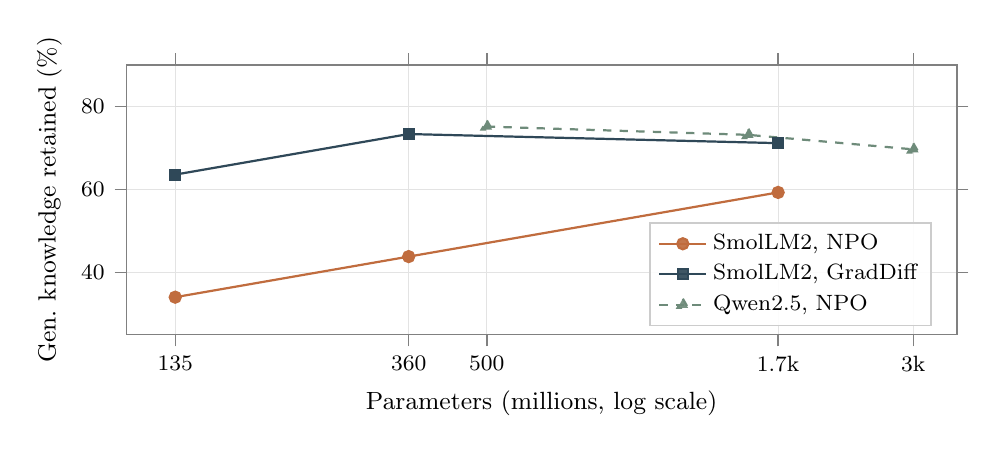
\begin{tikzpicture}
\begin{axis}[
  width=\columnwidth, height=5.0cm,
  xmode=log, log basis x=10,
  xlabel={Parameters (millions, log scale)},
  ylabel={Gen.\ knowledge retained (\%)},
  xtick={135,360,1700,500,3000}, xticklabels={135,360,1.7k,500,3k},
  ymin=25, ymax=90, xmin=110, xmax=3600,
  grid=both, legend pos=south east, legend cell align=left,
]
\addplot[inkB, thick, mark=*, mark size=2pt] coordinates {(135,34.0)(360,43.8)(1700,59.3)};
\addlegendentry{SmolLM2, NPO}
\addplot[inkA, thick, mark=square*, mark size=1.8pt] coordinates {(135,63.6)(360,73.4)(1700,71.2)};
\addlegendentry{SmolLM2, GradDiff}
\addplot[inkC, thick, dashed, mark=triangle*, mark size=2.2pt] coordinates {(500,75.2)(1500,73.2)(3000,69.7)};
\addlegendentry{Qwen2.5, NPO}
\end{axis}
\end{tikzpicture}
\caption{Collateral damage scales with model size. At a fixed forgetting level, smaller models retain less unrelated general knowledge. The effect is clean within SmolLM2 (both methods); Qwen2.5 under NPO is comparatively flat, which we discuss in \S\ref{sec:results}.}
\label{fig:scaling}
\Description{Line plot of retained general knowledge (percent) against model size on a log axis. For SmolLM2 under NPO, retention rises from 34 percent at 135M to 59 percent at 1.7B; GradDiff is higher and also increasing at the small end; Qwen2.5 under NPO stays roughly flat near 70 to 75 percent.}
\end{figure}

\begin{table}[t]
\centering
\caption{Baseline unlearning at matched forgetting. \emph{Ret.}\ is \texttt{world\_facts} retention (\% of pre-unlearning value); higher is better. The shaded column shows retention collapsing as SmolLM2 shrinks.}
\label{tab:diagnosis}
\small
\setlength{\arrayrulewidth}{0.3pt}
\begin{tabular}{llcc}
\toprule
\rowcolor{hiA} \textbf{Family} & \textbf{Size} & \textbf{GradDiff Ret.} & \textbf{NPO Ret.} \\
\midrule
\multirow{3}{*}{SmolLM2}
 & 135M & 63.6 & \cellcolor{inkB!22}\hurt{34.0} \\
 & 360M & 73.4 & \cellcolor{inkB!12}43.8 \\
 & 1.7B & 71.2 & \cellcolor{inkB!6}\keep{59.3} \\
\midrule
\multirow{3}{*}{Qwen2.5}
 & 0.5B & 55.4 & 75.2 \\
 & 1.5B & 69.5 & 73.2 \\
 & 3B   & 83.1 & 69.7 \\
\bottomrule
\end{tabular}
\end{table}

Figure~\ref{fig:scaling} and Table~\ref{tab:diagnosis} report the central finding. With the amount of forgetting held fixed, general-knowledge retention under NPO rises monotonically with scale across the SmolLM2 family---34\% at 135M, 44\% at 360M, 59\% at 1.7B---and the gradient-difference baseline shows the same ordering at the small end. A 135M model, forced to forget the same material to the same degree as its 1.7B sibling, gives up nearly two-thirds of its unrelated knowledge to do so.

The Qwen2.5 family complicates the picture rather than contradicting it. Its gradient-difference results follow the expected trend (55\%, 70\%, 83\%), but under NPO the three sizes sit close together and slightly inverted (75\%, 73\%, 70\%). Two factors contribute: the Qwen models began from stronger general knowledge, and their larger members were easier to over-forget near the stopping threshold. The consistent, clean signal is within SmolLM2; we take the honest reading to be that the effect is robust but not universal across every family and optimizer.

\begin{figure}[t]
\centering
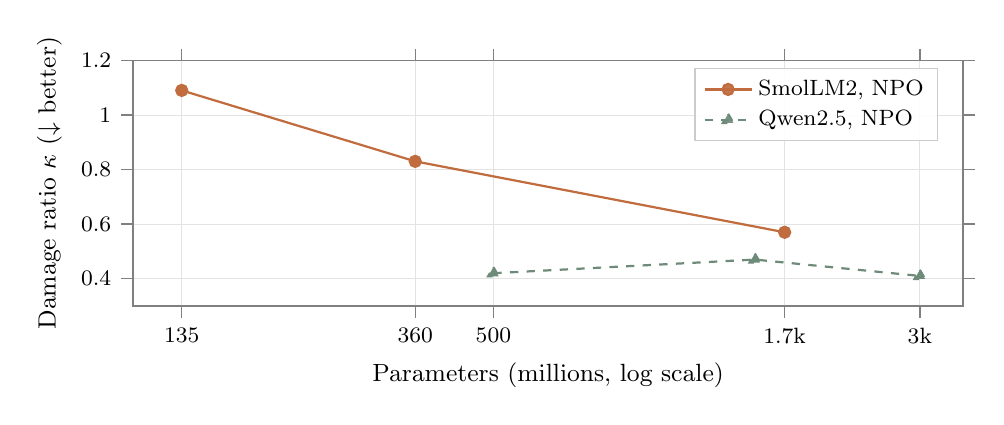
\begin{tikzpicture}
\begin{axis}[
  width=\columnwidth, height=4.7cm,
  xmode=log, log basis x=10,
  xlabel={Parameters (millions, log scale)},
  ylabel={Damage ratio $\kappa$ ($\downarrow$ better)},
  xtick={135,360,1700,500,3000}, xticklabels={135,360,1.7k,500,3k},
  ymin=0.3, ymax=1.2, xmin=110, xmax=3600,
  grid=both, legend pos=north east, legend cell align=left,
]
\addplot[inkB, thick, mark=*, mark size=2pt] coordinates {(135,1.09)(360,0.83)(1700,0.57)};
\addlegendentry{SmolLM2, NPO}
\addplot[inkC, thick, dashed, mark=triangle*, mark size=2.2pt] coordinates {(500,0.42)(1500,0.47)(3000,0.41)};
\addlegendentry{Qwen2.5, NPO}
\end{axis}
\end{tikzpicture}
\caption{Damage per unit of forgetting, $\kappa=(1-R)/E$ (Eq.~\eqref{eq:kappa}), which normalizes retention by how much each model actually forgot. Within SmolLM2 a 135M model loses nearly twice the general knowledge per unit forgotten as 1.7B. Qwen2.5 sits lower and flatter, consistent with its stronger base knowledge.}
\label{fig:kappa}
\Description{Line plot of the collateral-damage ratio kappa against model size on a log axis. For SmolLM2 under NPO, kappa falls from 1.09 at 135M to 0.57 at 1.7B; Qwen2.5 under NPO is lower and flatter near 0.4 to 0.47.}
\end{figure}

\paragraph{Damage per unit of forgetting.} The collateral-damage ratio $\kappa$ (Eq.~\eqref{eq:kappa}) sharpens the trend by normalizing out the small differences in how hard each model actually forgot. For SmolLM2 under NPO it falls from $\kappa{=}1.09$ at 135M to $0.83$ at 360M to $0.57$ at 1.7B (Figure~\ref{fig:kappa})---a 135M model destroys nearly twice as much general knowledge per unit of forgetting as its 1.7B sibling. The ordering is therefore not an artifact of the stopping band: it survives the normalization that $\kappa$ performs, which is the cleanest statement of the scaling effect we can make from the baselines alone.

\paragraph{The objective matters, too.} Table~\ref{tab:diagnosis} also shows that \emph{how} a model forgets shapes the damage. GradDiff retains more general knowledge than NPO at every scale---64\% versus 34\% at 135M---and the gap is widest at the small end. Part of this is that NPO, with its sharper preference gradient, tended to overshoot the stopping threshold before a probe could halt it; but the fact that the gentle and the aggressive forgetter diverge most where capacity is scarcest is itself consistent with the overlap picture. The lesson for a practitioner is that at small scale the choice of unlearning objective is not a detail---it is a first-order lever on how much unrelated knowledge survives.

\begin{figure}[t]
\centering
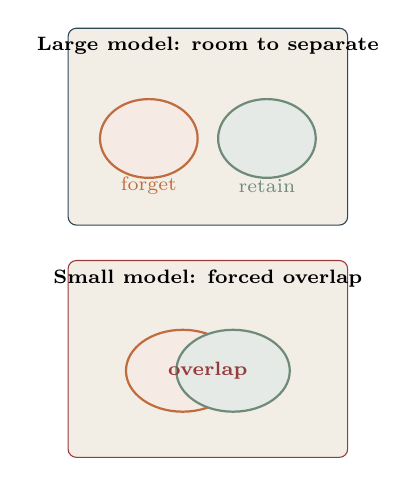
\begin{tikzpicture}[font=\footnotesize]
\def\panelw{3.55}
% ---- large model panel ----
\begin{scope}
\node[draw=inkA, rounded corners=3pt, fill=panel, minimum width=\panelw cm, minimum height=2.5cm] (L) {};
\node[anchor=north, font=\bfseries\scriptsize] at (L.north) {Large model: room to separate};
\draw[inkB, thick, fill=inkB!14] (-0.75,-0.15) ellipse (0.62 and 0.5);
\draw[inkC, thick, fill=inkC!18] (0.75,-0.15) ellipse (0.62 and 0.5);
\node[inkB, font=\scriptsize] at (-0.75,-0.75) {forget};
\node[inkC, font=\scriptsize] at (0.75,-0.75) {retain};
\end{scope}
% ---- small model panel ----
\begin{scope}[yshift=-2.95cm]
\node[draw=lock, rounded corners=3pt, fill=panel, minimum width=\panelw cm, minimum height=2.5cm] (S) {};
\node[anchor=north, font=\bfseries\scriptsize] at (S.north) {Small model: forced overlap};
\draw[inkB, thick, fill=inkB!14] (-0.32,-0.15) ellipse (0.72 and 0.52);
\draw[inkC, thick, fill=inkC!18] (0.32,-0.15) ellipse (0.72 and 0.52);
\node[lock, font=\scriptsize\bfseries] at (0,-0.15) {overlap};
\end{scope}
\end{tikzpicture}
\caption{Why the cost scales. In a large model the weights critical for the forget target and those critical for retained knowledge occupy largely separate regions, so an unlearning step disturbs little else. In a compact model, superposition forces them to share weights; removing the target drags retained knowledge with it. Fisher overlap between the two importance sets is high throughout our models ($\approx$\,0.6 Jaccard).}
\label{fig:capacity}
\Description{A two-panel schematic. The top panel, labelled large model, shows two separate ellipses for forget-critical and retain-critical weights with little overlap. The bottom panel, labelled small model, shows the same two ellipses overlapping heavily in a shared region.}
\end{figure}

\paragraph{Mechanism.} The scaling is consistent with capacity-driven overlap (Figure~\ref{fig:capacity}). For each model we computed the diagonal Fisher importance of every adapter weight separately for the forget and retain objectives and measured the overlap of their top-decile weights. The overlap is high throughout---roughly 0.6 by Jaccard---meaning the parameters most important for forgetting are largely the same ones most important for retaining.

To see that this is far from accidental, compare it to chance. For two independent top-$k$ importance sets drawn over $d$ effective directions, the expected Jaccard overlap is
\begin{equation}
\mathbb{E}[J] = \frac{k}{2d-k},
\end{equation}
which for top-decile sets ($k=0.1d$) is $\approx 0.053$. The measured $\approx 0.6$ is an order of magnitude above chance: the forget and retain objectives do not merely share a few weights, they concentrate on the \emph{same} directions. A compact model has fewer independent directions to spread facts across, so this coincidence can only grow as $d$ shrinks---the mechanical content of superposition. Its effect on unlearning is first-order: a step on the forget objective changes the retain loss by
\begin{equation}
\Delta\mathcal{L}_{\mathrm{retain}} \approx \eta\,\big\langle \nabla_\theta\mathcal{L}_{\mathrm{retain}},\ \nabla_\theta\mathcal{L}_{\mathrm{forget}}\big\rangle,
\label{eq:damage}
\end{equation}
and this inner product is large exactly when the two objectives' important directions align. Collateral damage is, to first order, the alignment between forgetting and retaining---and superposition drives that alignment up as models shrink.

\paragraph{What the damage looks like.} The metric hides the texture of the failure, so Figure~\ref{fig:qual} shows verbatim outputs. Forgetting itself is clean---the model stops reciting the target biography and confabulates a plausible substitute. The problem is next to it: unlearning one author also corrupts the identity of a \emph{different} author the model was asked to keep. The damage is not noise or gibberish; it is confident, fluent, and wrong, which is exactly what makes it dangerous.

\begin{figure}[t]
\begin{qbox}{Target to forget --- ``What is the full name of the author born in Taipei, Taiwan?'' (Qwen2.5-3B)}
\footnotesize
\textbf{Before:} \keep{``The author's full name is Hsiao Yun-Hwa.''}\\[1pt]
\textbf{After NPO:} ``Samantha Avery's books are inspired by her life\ldots''\\[1pt]
\textcolor{inkC}{\small$\Rightarrow$ forgetting succeeds: the target identity is gone.}
\end{qbox}
\vspace{2pt}
\begin{qbox}{Knowledge to keep --- ``Who are this author's parents?'' (a \emph{different}, retained author)}
\footnotesize
\textbf{Before:} ``Jaime Vasquez, son of a chef and a meteorologist\ldots''\\[1pt]
\textbf{After NPO:} \hurt{``Maria Luciahmena Tan delivers her stories\ldots''}\\[1pt]
\textcolor{lock}{\small$\Rightarrow$ collateral damage: an unrelated identity is overwritten.}
\end{qbox}
\caption{Collateral damage is fluent, not broken. Unlearning the Taipei author (top) also rewrites a retained author's identity (bottom). Outputs are verbatim; abbreviated for space.}
\label{fig:qual}
\Description{Two example boxes of verbatim model outputs. In the first, a query about the target author to be forgotten is answered correctly before unlearning and with a fabricated different name after NPO, showing forgetting succeeded. In the second, a query about a different author that should be retained is answered coherently before unlearning and with a wrong, unrelated identity after NPO, showing collateral damage.}
\end{figure}

% =====================================================================
\section{Method: Fisher-Masked NPO}
\label{sec:method}

\begin{figure}[t]
\centering
\begin{tikzpicture}[
  font=\footnotesize,
  box/.style={rounded corners=2pt, draw=inkA, line width=0.6pt, fill=panel, inner sep=4pt, align=center},
  gate/.style={rounded corners=2pt, draw=inkB, line width=0.8pt, fill=inkB!10, inner sep=4pt, align=center},
  flow/.style={-{Stealth[length=4pt]}, line width=0.6pt, draw=inkA!80},
]
\node[box] (df) {Forget set\\$\mathcal{D}_f$};
\node[box, below=4pt of df] (dr) {Retain set\\$\mathcal{D}_r$};
\node[gate, right=14pt of df] (fisher) {Fisher\\importance\\$F_r,\,F_f$};
\node[gate, right=14pt of fisher] (mask) {Keep-mask $M$\\protect retain-\\critical weights};
\node[box, below=26pt of mask, minimum width=3.2cm] (model) {LoRA model (frozen base)\\[1pt]
  \begin{tikzpicture}[baseline]
    \foreach \i/\c in {0/lock,1/inkC,2/lock,3/inkC,4/inkC,5/lock,6/inkC}{
      \fill[\c] (\i*0.32,0) rectangle (\i*0.32+0.22,0.28);
    }
  \end{tikzpicture}\\[-1pt]
  {\scriptsize \textcolor{lock}{$\blacksquare$}\,frozen \quad \textcolor{inkC}{$\blacksquare$}\,trainable}};
\node[box, left=14pt of model, minimum width=1.9cm] (loss) {NPO loss\\$\nabla_\theta \mathcal{L}_{\mathrm{NPO}}$};
\draw[flow] (df) -- (fisher);
\draw[flow] (dr.east) -- ++(6pt,0) |- (fisher.west);
\draw[flow] (fisher) -- (mask);
\draw[flow] (mask) -- (model);
\draw[flow] (df.south) -- ++(0,-6pt) |- (loss.north west);
\draw[flow] (loss) -- node[above, font=\scriptsize]{$\odot\,M$} (model);
\end{tikzpicture}
\caption{Fisher-Masked NPO. Diagonal Fisher importance on the retain and forget sets builds a keep-mask $M$ that freezes the weights most critical for retention (and not for forgetting). The NPO gradient is applied only through the unprotected weights.}
\label{fig:method}
\Description{Flow diagram of Fisher-Masked NPO. The forget and retain sets feed a Fisher-importance block, which builds a keep-mask that protects retain-critical weights. The NPO loss gradient is multiplied by this mask so that only unprotected weights of the LoRA model are updated while the frozen weights stay fixed.}
\end{figure}

Standard NPO minimizes a preference loss that drives the policy away from a reference model on the forget set, regularized by a retain-set term:
\begin{equation}
\mathcal{L}_{\mathrm{NPO}} = -\tfrac{2}{\beta}\,\mathbb{E}_{(x,y)\sim\mathcal{D}_f}\!\left[\log\sigma\!\left(-\beta\log\tfrac{\pi_\theta(y|x)}{\pi_{\mathrm{ref}}(y|x)}\right)\right] + \lambda\,\mathcal{L}_{\mathrm{CE}}(\mathcal{D}_r).
\end{equation}
The regularizer pulls back toward retained knowledge, but in a compact model it competes for the very weights the forget term is moving. We add a second, orthogonal defence: remove the most retention-critical weights from the optimization entirely.

For each adapter weight $w_i$ we accumulate the diagonal Fisher importance on the retain and forget sets,
\begin{equation}
F_i(\mathcal{D}) = \tfrac{1}{|\mathcal{D}|}\textstyle\sum_{(x,y)\in\mathcal{D}} \big(\partial \mathcal{L}_{\mathrm{CE}}(x,y)/\partial w_i\big)^2 .
\end{equation}
A weight is \emph{protected} when it is in the top $\alpha\%$ most important for retention and \emph{not} in the top $\alpha\%$ for forgetting---important to keep, and not needed to forget. The keep-mask $M$ is zero on protected weights and one elsewhere, and the update is masked,
\begin{equation}
\theta^{(t+1)} = \theta^{(t)} - \eta\,\big(M \odot \nabla_\theta \mathcal{L}_{\mathrm{NPO}}\big),
\end{equation}
realized with a gradient hook so protected weights never move (Figure~\ref{fig:method}). The intervention is cheap: Fisher scores are one backward pass per set, the mask is a boolean tensor, and nothing is added to inference. The one knob is $\alpha$, the protection strength.

\paragraph{Why the mask is the right choice.} The masked update freezes the protected set $P=\{i: M_i=0\}$: for $i\in P$, $\Delta\theta_i = -\eta M_i g_i = 0$. To first order the retain loss then moves by
\begin{equation}
\Delta\mathcal{L}_{\mathrm{retain}} \approx -\eta\sum_{i} M_i\, g_i\, \partial_i\mathcal{L}_{\mathrm{retain}},
\end{equation}
so every protected weight is dropped from this sum. Because $F_i(\mathcal{D}_r)=\mathbb{E}[(\partial_i\mathcal{L}_{\mathrm{retain}})^2]$ measures exactly how strongly weight $i$ can move the retain loss, freezing the top-$\alpha$ weights by $F_i(\mathcal{D}_r)$ removes the terms with the greatest potential to raise it. The exclusion $i\notin\mathrm{Top}_\alpha(F_f)$ keeps weights that forgetting genuinely needs unfrozen, so the forget budget is spent where it does not also carry retention. In this first-order sense the keep-mask is the optimal set of weights to immobilize: it minimizes the worst-case retain-loss increase at a fixed forgetting capacity. Connecting to Eq.~\eqref{eq:damage}, it severs the largest contributions to the forget--retain inner product, which is where the damage of \S\ref{sec:diagnosis} comes from.

\begin{algorithm}[t]
\caption{Fisher-Masked NPO}
\label{alg:fmnpo}
\small
\begin{algorithmic}[1]
\Require memorized model $\theta$; sets $\mathcal{D}_f,\mathcal{D}_r$; strength $\alpha$; forget target $\tau$; probe period $k$
\State $F_r \gets \textsc{FisherDiag}(\theta,\mathcal{D}_r)$;\quad $F_f \gets \textsc{FisherDiag}(\theta,\mathcal{D}_f)$ \Comment{one backward pass each}
\For{each adapter weight $i$}
  \State $M_i \gets 0$ \textbf{if} $i\in\mathrm{Top}_\alpha(F_r)\ \wedge\ i\notin\mathrm{Top}_\alpha(F_f)$, \textbf{else} $1$
\EndFor
\State register gradient hook $g \mapsto g\odot M$ on $\theta$
\Repeat
  \State $g \gets \nabla_\theta\,\mathcal{L}_{\mathrm{NPO}}(\mathcal{D}_f,\mathcal{D}_r)$;\quad $\theta \gets \theta - \eta\,(M\odot g)$
  \State \textbf{every $k$ steps:} \textbf{if} $\textsc{ForgetScore}(\theta)\le\tau$ \textbf{then break}
\Until{budget exhausted}
\State \Return unlearned model $\theta$
\end{algorithmic}
\end{algorithm}

\paragraph{Cost.} The procedure (Algorithm~\ref{alg:fmnpo}) adds only two Fisher passes over the LoRA parameters to an otherwise standard NPO run, so memory stays negligible even at 3B and nothing is added at inference. With the settings of Table~\ref{tab:config}, the entire study---six models, three unlearning methods, and the ablations---runs in a few GPU-hours on a single A100.

% =====================================================================
\section{Experiments and Results}
\label{sec:results}

\begin{figure}[t]
\centering
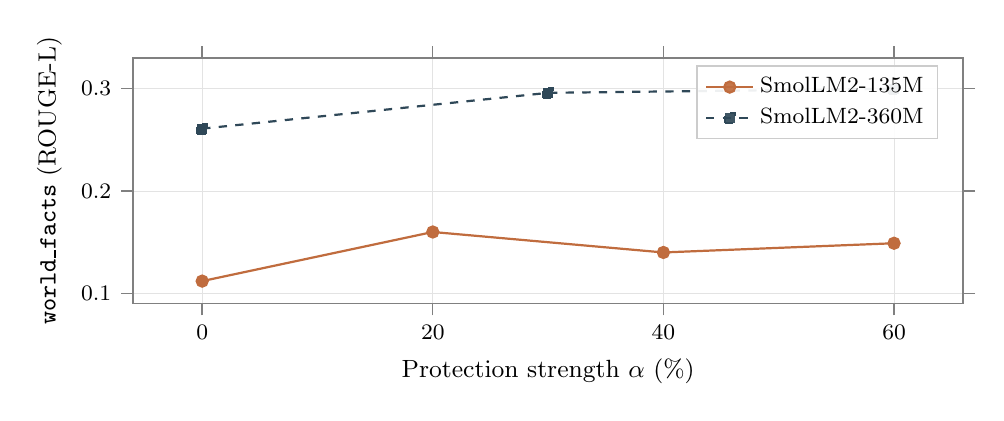
\begin{tikzpicture}
\begin{axis}[
  width=\columnwidth, height=4.7cm,
  xlabel={Protection strength $\alpha$ (\%)},
  ylabel={\texttt{world\_facts} (ROUGE-L)},
  xtick={0,20,40,60}, ymin=0.09, ymax=0.33,
  grid=both, legend pos=north east, legend cell align=left,
]
\addplot[inkB, thick, mark=*, mark size=2pt] coordinates {(0,0.112)(20,0.160)(40,0.140)(60,0.149)};
\addlegendentry{SmolLM2-135M}
\addplot[inkA, thick, dashed, mark=square*, mark size=1.8pt] coordinates {(0,0.261)(30,0.296)(60,0.300)};
\addlegendentry{SmolLM2-360M}
\end{axis}
\end{tikzpicture}
\caption{Controlled mask ablation: same model, same forgetting level, only $\alpha$ changes. Turning the mask on ($\alpha{>}0$) raises retained knowledge over the unmasked baseline ($\alpha{=}0$) at both scales---$+43\%$ relative at 135M, $+15\%$ at 360M. This is the cleanest, confound-free evidence that the protection works.}
\label{fig:ablation}
\Description{Line plot of world_facts retention (ROUGE-L) against mask strength alpha for two small models. For SmolLM2-135M retention rises from 0.112 at alpha zero to about 0.16 once the mask is on; for SmolLM2-360M it rises from 0.261 to about 0.30, showing that turning the mask on improves retention at a fixed forgetting level.}
\end{figure}

\begin{table}[t]
\centering
\caption{Fisher-Masked NPO vs.\ NPO at matched forgetting ($\alpha{=}50\%$). Retention is \% of pre-unlearning \texttt{world\_facts}. The $\Delta$ column is shaded by sign: a single fixed mask helps at some scales and hurts at others.}
\label{tab:fmvsnpo}
\small
\begin{tabular}{lccc}
\toprule
\rowcolor{hiA} \textbf{Model} & \textbf{NPO Ret.} & \textbf{FM-NPO Ret.} & \textbf{$\Delta$} \\
\midrule
SmolLM2-135M & 34.0 & 35.5 & \cellcolor{good!18}$+1.5$ \\
\rowcolor{hiB} SmolLM2-360M & 43.8 & 29.1 & \cellcolor{lock!20}$-14.6$ \\
SmolLM2-1.7B & 59.3 & 58.5 & \cellcolor{lock!8}$-0.8$ \\
\rowcolor{hiB} Qwen2.5-0.5B & 75.2 & 47.2 & \cellcolor{lock!28}$-28.0$ \\
Qwen2.5-1.5B & 73.2 & 75.2 & \cellcolor{good!18}$+2.0$ \\
\rowcolor{hiB} Qwen2.5-3B   & 69.7 & 73.8 & \cellcolor{good!26}$+4.1$ \\
\bottomrule
\end{tabular}
\end{table}

\paragraph{The mask reduces collateral damage (controlled).} Figure~\ref{fig:ablation} is the result we trust most, because it removes every confound: a single model, unlearned to a single forgetting level, with only $\alpha$ varied. At 135M, turning the mask on lifts retained general knowledge from 0.112 to 0.160 ROUGE-L, a 43\% relative gain; at 360M it rises from 0.261 to 0.300, a 15\% gain. Protecting retention-critical weights demonstrably buys back knowledge that unlearning would otherwise destroy, and it does so most at the smallest, most capacity-pressed scale---exactly where Section~\ref{sec:diagnosis} said the damage is worst. The curve is not perfectly monotone in $\alpha$ (135M peaks near $\alpha{=}20$), which already signals that the optimal protection strength is model-specific.

\paragraph{A fixed global mask is not a uniform win.} Table~\ref{tab:fmvsnpo} is the honest counterweight. Fixing $\alpha{=}50\%$ for every model and comparing against plain NPO at matched forgetting, the benefit ranges from $+4\%$ to $-28\%$: it helps the smallest SmolLM2 model and the larger Qwen models, and it hurts the 360M and 0.5B cases. The ablation and this table are not in conflict---the first compares the mask against \emph{itself} at $\alpha{=}0$ on one model, the second compares a \emph{single} mask strength against a differently-tuned baseline across heterogeneous models. Read together, they say the mechanism is real but the operating point must be chosen per model; a strength that protects the right amount at one scale over-constrains or under-constrains another.

\paragraph{Choosing the protection strength.} The ablation (Figure~\ref{fig:ablation}) exposes the practical difficulty directly: the best $\alpha$ is not shared across scales. On the 135M model retention peaks near $\alpha{=}20\%$ and then declines, while on the 360M model it keeps rising through $\alpha{=}60\%$. The reading is intuitive---the smaller model has fewer retention-critical weights to spare, so protecting too many of them starves the forget objective of room to work, whereas the larger model tolerates, and benefits from, more protection. A fixed global $\alpha$ therefore cannot be optimal everywhere, which is exactly what Table~\ref{tab:fmvsnpo} reflects. A cheap heuristic suggests itself: set $\alpha$ from the measured forget--retain Fisher overlap, protecting more where overlap is higher. The ingredient---the per-model overlap---is already computed to build the mask.

\paragraph{Takeaway.} The protection is an effective lever, not yet a universal recipe. The controlled evidence for the mechanism is solid; turning it into a method that improves every model out of the box requires making $\alpha$ adaptive, which we outline next.

\paragraph{Reproducibility.} Every result follows the single matched-forgetting protocol of \S\ref{sec:setup}, with the same seed, the same stopping threshold, and a single final evaluation per run. We release the memorized base checkpoints for all six models, the Fisher importances used to build the masks, and the notebooks that reproduce every table and figure from them, so that the baselines, the mask, and the ablations can be re-run or re-tuned without recomputation. Code and notebooks are available at \url{https://github.com/Codewithsayanjib/like-a-childs-mind}.

% =====================================================================
\section{Discussion and Limitations}
Three findings stand out. \emph{(i)} At matched forgetting, collateral damage to general knowledge grows as models shrink---cleanly within SmolLM2 and quantified by the damage ratio $\kappa$, which nearly doubles from 0.57 at 1.7B to 1.09 at 135M. \emph{(ii)} The damage is mechanistic: forget- and retain-critical weights overlap an order of magnitude above chance, so the two objectives share directions and an unlearning step moves both (Eq.~\eqref{eq:damage}). \emph{(iii)} Freezing retain-critical weights reduces the damage in controlled comparisons, most at the smallest scale, though a single global $\alpha$ is not yet uniformly optimal. We now set the boundaries of these claims.

We studied two families and three scales each; the clean monotone trend is clearest within SmolLM2, and Qwen2.5 under NPO is comparatively flat, so the scaling claim is well-supported but not demonstrated to be family-independent. Our matched-forgetting stop probes frequently but still lands in a small band rather than an exact point, which contributes noise to the cross-model comparison in Table~\ref{tab:fmvsnpo}. The Fisher mask has a single global strength $\alpha$; the ablation shows the best value is scale-dependent, and we did not tune it per model. Finally, we evaluate with ROUGE-L on TOFU-style probes; stronger forget-quality and membership-inference metrics would sharpen the forgetting side of the comparison. This limit is partly fundamental: approximate unlearning cannot be certified from a model's weights alone, since the same weights can arise from different data~\cite{thudi}, so behavioural and membership tests---not weight inspection---are the practical standard of evidence, and our retention measure should be read as a utility diagnostic rather than a certificate of erasure. None of these undercut the central, controlled finding---that protecting retention-critical weights reduces collateral damage---but they bound how far the fixed-$\alpha$ method should be read as a solved solution.

\paragraph{Toward an adaptive mask.} Three extensions follow directly from the analysis. First, make $\alpha$ adaptive---chosen per model from the Fisher overlap, or set per layer to protect more in the middle layers where superposition tends to concentrate. Second, replace the binary mask with a soft one that scales each gradient by a continuous function of importance, removing the hard cliff at the $\alpha$ threshold that the non-monotone ablation curve hints at. Third, pair the method with membership-style recovery probes, so that reduced collateral damage is never bought with weaker forgetting. Each keeps the one-backward-pass cost that makes the approach attractive at small scale.

\paragraph{Broader impact.} Small on-device models are precisely the ones to which deletion requests will increasingly apply, and precisely the ones that unlearning damages most. That raises a double risk: a deletion that quietly degrades the model, and a deletion that \emph{appears} to succeed while the fact remains recoverable. Capacity-aware unlearning addresses the first; the second argues for pairing any such method with adversarial recovery tests before a deletion is certified.

% =====================================================================
\section{Conclusion}
Unlearning does not scale down for free. Holding the amount of forgetting fixed, compact language models pay a steeper price in general knowledge than larger ones, and the cost tracks the overlap between the weights that store a fact and the weights that keep the model capable. Freezing the most retention-critical weights with a cheap Fisher mask provably reduces this cost in controlled comparisons, most at the smallest scale---though a single fixed protection strength is not yet a uniform improvement. For the small models that privacy law will increasingly target, capacity-aware unlearning is both necessary and, we show, tractable in principle.

% =====================================================================
\bibliographystyle{ACM-Reference-Format}
\bibliography{references}

\end{document}
